\chapter{绪论}
\label{chap:intro}
近几十年来,随着半导体技术的不断发展,计算机系统的性能成几何级增长。
一方面,由于半导体工艺的不断进步,晶体管尺寸不断缩小,芯片能够集成的晶体管数目不断增大;
另一方面,也是因为硬件系统结构、编译技术和算法的不断发展和进步。
在这些性能增长中,晶体管尺寸的缩减起到了决定性作用~\upcite{hennessy2011computer}。
然而,从2005年开始,量子隧穿效应使得晶体管漏电现象开始出现。
晶体管尺寸由于受到小晶体管静态功耗的影响,已经难以再按照登纳德缩放比例定律(Dennard Scaling)~\upcite{dennard1974design}继续缩减,
时钟频率难以继续提升。
为了继续提升性能,就必须从更高效的体系结构上下功夫。多核处理器、配有专用硬件加速器的异构系统应运而生。

研究发现,专用硬件加速器能够显著提升处理器的能效比~\upcite{hameed2010understanding}。 
无论是传统的DSP~\upcite{chen2014ft}、GPU~\upcite{volta, pascal, fermi, amd-fusion, radeon},还是针对深度神经网络加速的谷歌TPU~\upcite{Jouppi:2017:IPA:3079856.3080246}、寒武纪AI加速器~\upcite{chen2014diannao,chen2014dadiannao},这些加速器与CPU组成异构系统。
该体系结构通过将大量并行计算或专用计算任务从CPU发送到GPU、DSP或其他专用加速器,显著减少了CPU指令执行的开销和程序员的负担,系统性能和能效均显著提高,
对于图像处理、高性能计算、以及深度学习训练~\upcite{krizhevsky2012imagenet,simonyan2014very,szegedy2015going,zeiler2014visualizing}都具有重要作用。
在这之中,GPU处理器的应用最为广泛,据Hameed等人的研究表明,一个GPU的运算处理性能通常不低于10个CPU核~\upcite{hameed2010understanding}。
虽然起初其出现的主要目标是解决CPU对图像渲染加速不足的问题,但由于其架构在处理并行计算的天然优势,使得GPU目前更多地被用于通用并行计算~\upcite{bolz2003sparse,fan2004gpu,he2008mars}。
如今无论是手机、平板电脑、笔记本,还是数据中心和超级计算机,GPU已无处不在。

异构系统不断发展,应用规模和数据规模不断增长,又遇到了存储墙问题,访存开销越来越大。
在此背景之下,为了继续维持摩尔定律,提升集成电路性能的同时降低集成电路的开销,\texttt{集成电路堆叠技术}~\upcite{Xie:2015:DA:2842825,loh-ieeemicro2007, samsung-pr2007,black2013stacking}成为一种有效解决方案被广泛应用。
三维堆叠集成技术是一种新的集成电路工艺,将多个硅片垂直堆叠并以三维封装的方式封装成一个芯片,
是在工艺尺寸缩减受限的情况下提高系统性能的一种新的方式。
三维堆叠集成电路技术从\texttt{延伸摩尔定律}和\texttt{超越摩尔定律}两方面实现芯片上晶体管密度和芯片性能的大幅度提升,
在提升带宽、降低延迟和提高能效方面有许多优势。不过,受限于良率、热效应、设计复杂度、设计测试成本以及EDA工具等方面的限制,
三维堆叠技术目前主要用于一些如存储器等互连简单、单元排列重复的规则电路。
相比于三维堆叠技术这种革命性的革新,\texttt{基于硅中介层的2.5维堆叠技术}则属于一种进化技术,避免了三维堆叠技术中的各种问题。
2.5维堆叠集成电路是将多个同构或异构的部件相邻地堆叠在硅中介层上,相邻部件之间通过硅中介层进行通信。
通过2.5维堆叠可以将处理器和三维堆叠存储器相邻地堆叠在硅中介层上,为处理器增加内存容量的同时显著提高内存带宽,已经广泛用于目前商业化的异构处理器中。


\section{研究动机}
高性能堆叠异构系统目前已经被引入数据中心,为云计算~\upcite{mell2011nist,dillon2010cloud,hauswald2015sirius}提供更加强大的计算和存储能力。
云计算中\texttt{多租户技术}的应用使得多个用户能够共享高性能堆叠异构处理器,并同时执行和处理多个任务。
无论是\texttt{IaaS}~\upcite{bhardwaj2010cloud}、\texttt{PaaS}~\upcite{vaquero2008break}、还是\texttt{SaaS}~\upcite{koomey2011growth},均对多租户技术有着强烈的需求。
多租户任务允许计算资源的共享和存储资源的相互隔离,同时需要保证多租户任务间的安全隔离性。
虽然多租户技术保证了安全隔离性,但用户无法了解任务运行的具体情况,难以从程序员的角度对应用程序进行优化,
因此,研究面向堆叠异构系统的应用透明策略显得尤为重要。

本文从堆叠异构系统出发,发现并解决堆叠异构系统的三大问题:

\textbf{内存超额配置造成的性能骤降问题。}
云提供商往往会给用户提供超过其硬件资源的存储资源,在用户不同时使用这些资源的情况下提高数据中心的资源利用率。
然而随着用户应用规模和数据量的不断增大,内存超额配置越来越普遍。
堆叠异构处理器,如GPU,目前已经能够为用户提供内存超额配置的支持。
但通过我们在真实GPU的实验发现,当内存超额配置时,GPU出现了严重的性能下降,在一些情况下甚至会发生宕机。

\textbf{多任务抢占的高上下文切换开销问题。}
为在多任务处理中快速响应一些优先级较高,对延迟比较敏感的任务,必须支持多任务抢占机制进行快速切换。
上下文切换是多任务抢占的一种重要方式。
然而GPU等堆叠异构系统相对于CPU,由于其同时处理大量数据,上下文大小相对较大。
因此,GPU上下文切换的开销远大于CPU,传统的上下文切换机制占用的存储带宽将严重影响多任务抢占的性能。

\textbf{堆叠互连网络结构的负载不均衡问题。}
在2.5维堆叠异构系统中,传统的方式是在相邻处理器或存储器的四周边缘通过硅中介层进行互连。
Enright Jerger等人~\upcite{jerger2014noc}提出利用硅中介层大量的连线资源设计了2.5维片上互连网络。
一般情况下,该网络结构通过上层网络进行一致性协议报文的通信,通过下层网络进行访存报文的通信。
但是,我们的实验发现,由于不同类型报文的不均衡性,该方法会导致上下层网络的负载不均衡问题,严重影响整个系统的性能。

本文的研究发现,传统的通过程序员手工调试优化的技术都难以在支持多租户技术数据中心中高效使用。
本文针对堆叠异构系统中的上述三大问题,研究对应用透明的硬件或驱动策略,
使得堆叠异构系统能够在程序员不修改应用程序的前提之下为这些问题提供高效的解决方案。

\section{研究内容和主要贡献}

\subsection{研究内容}
本文面向堆叠异构系统,研究对应用透明、程序员不感知的优化策略,解决上述三大问题,主要包括:

(1)一种内存超额配置管理策略框架(ETC)

现代分立式GPU支持统一内存技术和实时按需取页技术。这种在CPU和GPU内存中自动的数据拷贝管理显著降低了开发者的负担。
但是,当应用程序的在线工作数据集超过GPU物理内存时,产生的额外数据移动会导致严重的性能损失。

本文提出了一种内存超额配置管理框架(ETC),采用了一系列对应用和程序员透明的新技术提升内存超额配置下的GPU性能。
主要思想包括掩藏数据页逐出延迟、降低内存抖动开销、以及增大有效的内存空间。
数据页逐出延迟可以通过\texttt{主动数据页逐出技术}尽早为将要取进来的数据页腾出空间,掩藏延迟;
内存抖动的开销可以通过\texttt{内存感知的并行度控制策略},动态地将GPU的并行度降低以减少在线工作数据集的大小,缓解内存抖动现象;
\texttt{内存容量压缩技术}在不需要增大物理内存容量的前提下使得更大的在线工作数据集能够被内存容纳。
本章发现没有任何一种技术对所有类型的应用程序都有效。因此,ETC将\texttt{主动数据页逐出技术}、\texttt{并行度控制策略}和\texttt{内存容量压缩技术}
集成到一个管理框架,当内存超额配置时针对应用程序类型动态地选择这些策略的组合,对应用程序透明的提升GPU的性能。
从这个角度出发,ETC将应用程序划分为无数据共享的规则应用程序、数据共享的规则应用程序以及不规则的应用程序。

实验分别实现了一种当前的基准结构、一种具有无限内存大小的理想结构以及ETC。
ETC几乎能够完全消除无数据共享的规则应用程序的内存超额配置开销,使之性能与具有无限内存空间的理想情况类似。
本章还发现,相比于当前的基准策略,ETC能够将数据共享的规则应用程序和不规则应用程序的内存超额配置开销显著降低。

(2)一种动态采用检查点备份技术的GPU主动抢占策略(PEP)

无论是空间上的多任务支持还是时间上的多任务支持,GPU对多任务处理的需求都在不断增加。
这要求GPU可以随时被高优先级应用程序抢占,在某一应用程序正在执行的过程中,中断执行并切换上下文到新的应用程序。
不同于CPU,GPU由于其大量的上下文大小,上下文切换产生的开销非常大。
研究人员已经做出了大量工作来降低GPU上的抢占开销。
例如降低上下文的大小或将上下文切换和程序执行重叠等。
而所有之前的这些方法都是被动式的,意味着上下文切换都是在抢占请求到来之后才开始的。

本文提出了一种动态主动的抢占机制(PEP)来降低抢占的延迟,本文观察到GPU内核函数的执行无论是在CUDA还是OpenCL下都一定是在内核函数启动后开始的。
因此,抢占请求可以在其实际到达GPU前预测。本文研究了这一段延迟,并开发了一种预测机制提前进行状态备份。
当抢占请求实际到达GPU后,只需要将相对于上一次状态备份的增量部分再做备份,非常类似于传统的检查点备份技术。
本文的设计同时也可以根据GPU内核函数在运行过程中的特性动态选择\texttt{排空执行技术}或\texttt{基于检查点的上下文备份技术}。
实验测试结果表明,PEP设计可以有效的降低等待上下文切换产生的停滞延迟。
此外,PEP的脏上下文备份机制也有效地减少了需要备份的上下文的大小。

(3)一种动态延迟感知的2.5维堆叠片上网络负载均衡策略(DLL)

由于三维堆叠技术依然面临许多的挑战,当前2.5维堆叠技术具有更好的应用前景。
通过硅中介层的应用,2.5维堆叠技术可以为异构处理器提供更高带宽和更大容量的存储系统。
为了满足2.5维堆叠芯片的存储系统通信要求,可以硅中介层上丰富的连线资源可以来开发并实现一套新的网络。
但是,实验发现2.5维堆叠片上网络体系结构的性能受到两层网络之间严重的不均衡负载限制,难以发挥出应有的性能。

为了解决这个问题,本文提出了一种动态延迟感知的负载均衡策略(DLL)。
核心想法是通过最近几个报文的平均延迟来检测整个网络层的拥塞程度,
根据收集到的数据在每个源节点进行报文网络层的路由选择。
我们利用了硅中介层上充足的连线资源实现了一个延迟传播环网,
确保在目的节点收集到的报文延迟信息能够传输回源节点,
采用这些信息进行路由选择达到了负载均衡的目标。

实验将DLL策略的实现与无负载均衡策略的基准设计、一种目的节点检测的策略和一种缓存感知的策略的实现进行比较,
我们的DLL策略均达到了吞吐率提升,同时产生的开销非常小。


\subsection{主要贡献}
本文系统深入地研究了应用透明策略以提升堆叠异构系统的性能,取得了许多系统性开创性的成果,主要创新点如下:

(1)提出了一种内存超额配置的管理框架

内存超额配置虽然在当前GPU中得到了完全支持,但之前的工作没有考虑内存超额配置所带来的严重开销,
且内存超额配置的优化工作都需要修改应用程序,难度较大且效果不一定好。
本文提出了一种内存超额配置的管理框架,主要贡献包括:
\renewcommand*\theenumi{(\alph{enumi})}
\begin{enumerate}
\setlength\itemsep{1pt}
\item 据我们所知,这是第一个对GPU内存超额配之下的性能开销做深度分析的工作。
通过对应用程序访存trace的分析,找出了不同应用程序类型在GPU内存超额配置下出现严重性能损失的不同原因。
\item 提出了一种软硬件结合的对应用透明的解决方案,能够显著降低内存超额配之下的性能损失。
该方法对程序员不感知,不需要任何应用程序代码的修改。
\item 开发了三种内存超额配置的优化策略。我们发现并没有任何一种单一方法能够对所有类型的应用程序都见效。
从这个角度出发,本研究的策略根据访存特性,在线划分应用程序的类别,并为不同类别的应用程序采用不同的策略组合进行性能优化。
\end{enumerate}

该部分的研究成果~\upcite{Li:asplos19}发表在系统结构领域的顶级会议第24届ACM国际编程语言与操作系统的体系结构支持会议
(The 24th ACM International Conference on Architectural Support for Programming Languages and Operating Systems, ASPLOS-19)上。

(2)提出了一种动态采用检查点备份技术的GPU主动抢占策略

GPU中的多任务抢占开销非常大,这是由于相对于CPU,GPU的上下文较多,需要备份的上下文数据较大。
传统的抢占方案都采用了被动方法,即抢占请求到来时才开始上下文切换。
本文开创性的采用了主动抢占方法,提出了一种动态采用检查点备份技术的GPU主动抢占策略,主要贡献包括:
\renewcommand*\theenumi{(\alph{enumi})}
\begin{enumerate}
\setlength\itemsep{1pt}
\item 研究了GPU内核函数的启动过程,观察到抢占请求可以被提前预测到。
\item 引入了一种主动的抢占技术来减少抢占内核函数等待上下文切换的时间。
通过采用检查点备份技术,当实际抢占请求到来时,只有需要存储一小部分更新的上下文。
\item 使用了一种相对简单的脏数据存储技术来减少上下文大小,从而减少不必要的上下文存储开销。
\item 开发了一种更加精确的线程块执行时间和上下文切换时间的估算方法,设计了实时动态选择算法以确定采用不同抢占方法的时机。
我们可以分别完成长短内核函数的抢占,并使之实现最短延迟和最小开销。
\end{enumerate}

该研究的部分成果~\upcite{Li:dac18}发表在了计算机辅助设计领域顶级会议第55届设计自动化国际会议
(The 55th Design Automation Conference, DAC-18)上,
完整内容~\upcite{li2018dynamic}发表在了体系结构旗舰期刊IEEE Transactions on Computer-Aided Design of Integrated Circuits and Systems上。 

(3)提出了一种动态延迟感知的2.5维堆叠片上网络负载均衡策略

2.5维堆叠片上网络作为一种全新的网络结构目前的研究还不多。
由于其特有的网络通信特征,传统的多层网络结构以及三维堆叠片上网络方法难以直接应用到2.5维堆叠片上网络结构上。
本研究发现之前的2.5维片上网络研究未考虑到均衡负载的问题。
针对该问题,本文研究了一种动态延迟感知的2.5维堆叠片上网络负载均衡策略,主要贡献包括:
\renewcommand*\theenumi{(\alph{enumi})}
\begin{enumerate}
\setlength\itemsep{1pt}
\item 评估并分析了PARSEC测试集的通信流量,发现2.5维堆叠片上网络的通信流量在两个网络层极不公平。
\item 分析了当前负载均衡策略的缺点。缓存感知的方法无法获取全局网络的拥塞情况;当前的延迟感知方法不能准确地检测全局拥塞状态。
根据这些不足,本文提出了一种应用偷摸的延迟感知方法均衡负载。
\item 设计了一个多链路无阻塞环网,通过该环网,将目的节点收集的拥塞信息传输回源节点用于网络选择。
\end{enumerate}

该部分的研究成果~\upcite{li2016dll}发表在了第34届国际计算机设计会议(The 34th IEEE International Conference on Computer Design, ICCD-16)上。

\section{研究框架概述}

本文研究了堆叠异构系统的三大问题,包括异构系统的内存墙问题、多任务切换的抢占问题、以及堆叠互连网络的负载均衡问题。
如图~\ref{fig:structure}所示,本文提出了三种对应用透明的软硬件策略,能够有效解决堆叠异构系统的三大问题,使其缓解内存超额配置带来的严重性能损失、
降低堆叠异构系统多任务调度的上下文切换延迟、以及均衡堆叠互连网络的负载等。
上述应用透明策略均在模拟器中得到了有效验证。

\begin{figure}[htbp] % use float package if you want it here
  \centering
  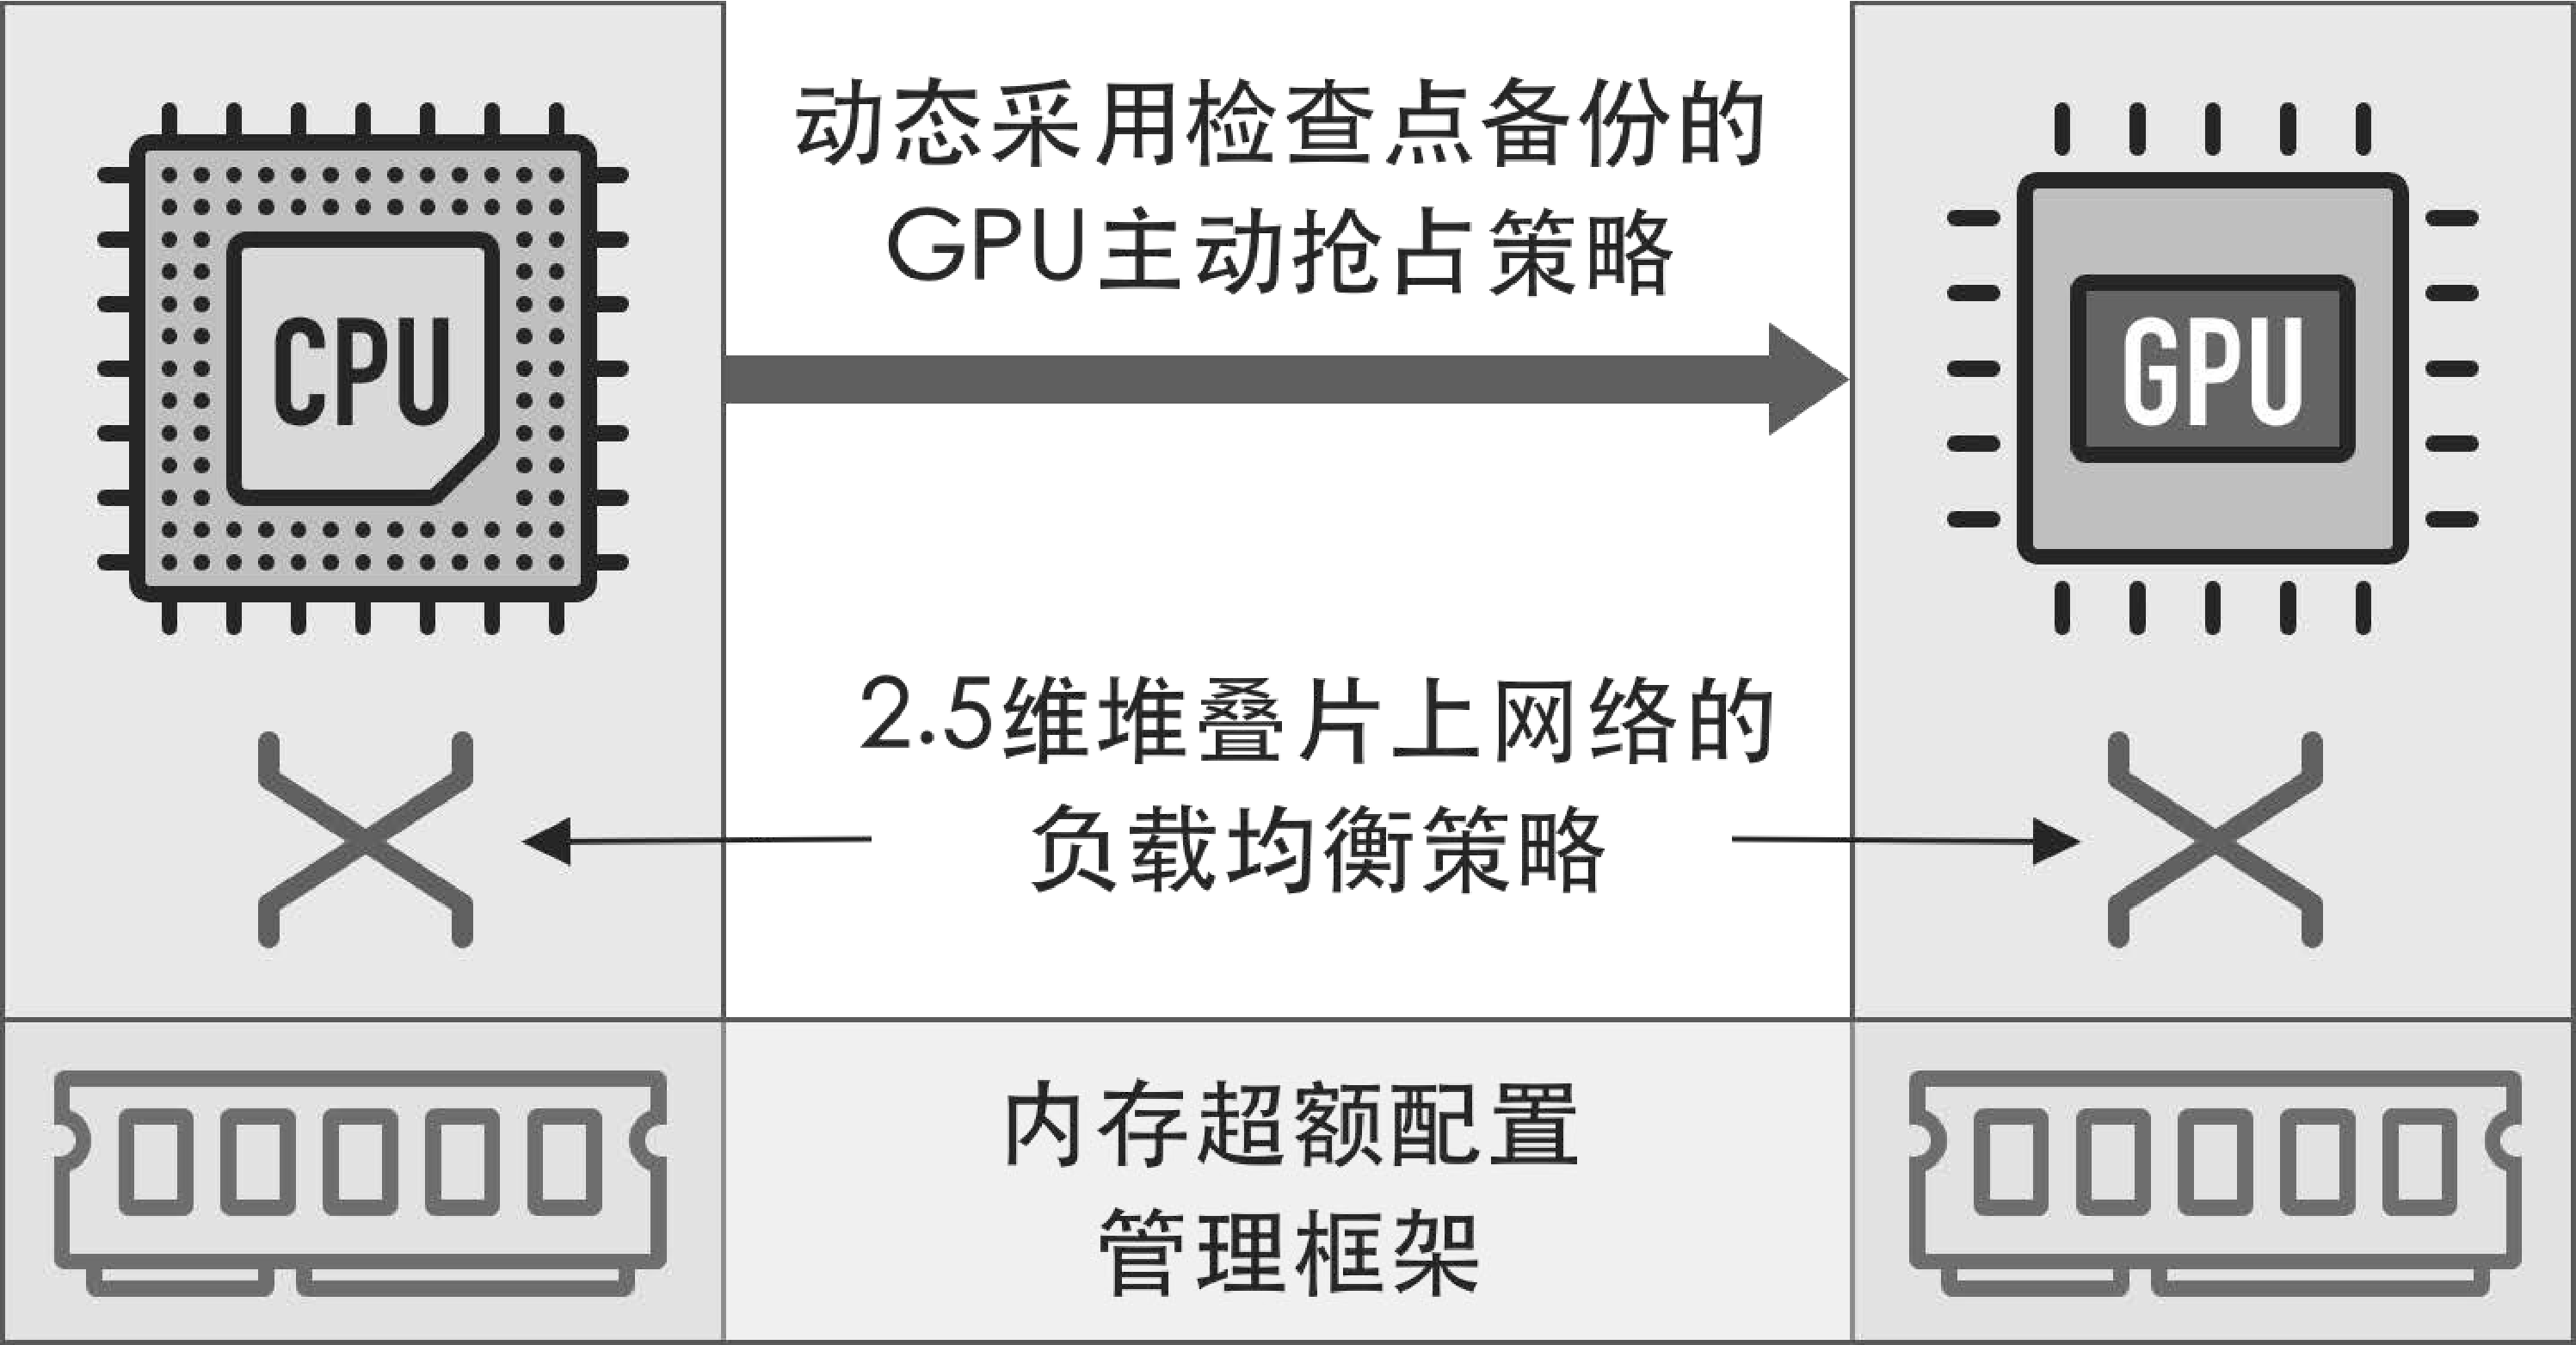
\includegraphics[width=0.7\textwidth]{/Figs_Intro/structure}
  \caption{研究框架概述}
  \label{fig:structure}
\end{figure}

如图~\ref{fig:structure}所示,应用透明的软硬件策略包括:\texttt{面向CPU-GPU统一虚拟内存的内存超额配置管理框架},解决异构系统的内存超额配置问题;
\texttt{动态采用检查点备份的主动抢占策略},解决多任务切换时抢占延迟过高的问题;
以及\texttt{面向2.5维堆叠片上网络的负载均衡策略},解决两层网络负载不均衡的问题。
这三个研究点系统地分析了堆叠异构系统的内存管理、任务调度以及互连网络存在的问题,根据问题出现的原因提出了相应的应用透明解决策略。
应用透明的策略可以适应租户对数据中心系统运行不敏感的特点,在不增加程序员负担的同时,从软硬件结合的角度有效提升了异构系统的性能。


本文解决的三大问题主要位于堆叠异构系统的应用调度、网络和存储三部分。
这三部分相互独立,但并不冲突。
这些应用透明策略的共同应用,有助于缓解堆叠异构系统在不同层次的瓶颈,提升堆叠异构系统的性能。
在数据中心系统中,有助于优化多租户下的系统性能,同时对程序员的要求较低。




\section{论文组织结构}
本文紧紧围绕堆叠异构系统结构,对应用透明的架构和调度策略进行深入研究。
本文共分六章,按以下方式组织:
第~\ref{chap:intro}章为绪论,介绍了本文的研究动机以及相关研究内容和创新点;
第~\ref{chap:background}章从堆叠系统、GPU架构和异构系统相关策略优化三个方面介绍了本文的研究背景和相关基础;
第~\ref{chap:ETC}章介绍了针对GPU内存超额配置所提出的应用透明框架;
第~\ref{chap:PEP}章介绍了面向堆叠异构系统的多任务切换提出的基于动态检查点备份的优化方案;
第~\ref{chap:DLL}章介绍了针对2.5维堆叠片上网络结构提出的延迟感知的负载均衡策略;
第~\ref{chap:conclusion}章对全文进行了总结,并展望下一步工作。
